\subsection{Implementacja oraz dobór nastaw dwupętlowego regulatora PID}
\label{lab:zad3}


Na	sterowniku	zaimplementowano	uwzględniając	ograniczenia	dwupętlowy	
regulator	PID. Wyznaczając model dobrano nastawy regulatora.

\subsubsection{Implementacja regulatora PID}

\ifdefined\CompileListings
    \lstinputlisting[
        firstline=34, 
        lastline=47, 
        caption="Inicjacja parametrów regulatora PID toru G1-T1"]
        {../lab/src/Init_Initial.st}
    %\newpage
\fi

\ifdefined\CompileListings
    \lstinputlisting[
        firstline=49, 
        lastline=62, 
        caption="Inicjacja parametrów regulatora PID toru G2-T3"]
        {../lab/src/Init_Initial.st}
    \newpage
\fi

\ifdefined\CompileListings
    \lstinputlisting[
        firstline=3, 
        lastline=46, 
        caption="Program regulatora PID toru G1-T1"]
        {../lab/src/PID_R_FixedScan.st}
    \newpage
\fi

\ifdefined\CompileListings
    \lstinputlisting[
        firstline=48, 
        lastline=91, 
        caption="Program regulatora PID toru G2-T3"]
        {../lab/src/PID_R_FixedScan.st}
\fi
\newpage
\subsubsection{Dobranie nastaw regulatora}

Metodą eksperymentalną etapami dobrano nastawy regulatorów PID.
\newline
Przyjęto takie same nastawy dla obydwu regulatorów.

$$Kr = \num{15.0} \indent Ti = \num{250.0} \indent Td = \num{0.001}$$

\ifdefined\CompileFigures
\begin{figure}[H] 
    \centering
    % This file was created by matlab2tikz.
%
\definecolor{mycolor1}{rgb}{0.00000,0.44700,0.74100}%
\definecolor{mycolor2}{rgb}{0.85000,0.32500,0.09800}%
\definecolor{mycolor3}{rgb}{0.92900,0.69400,0.12500}%
\definecolor{mycolor4}{rgb}{0.49400,0.18400,0.55600}%
%
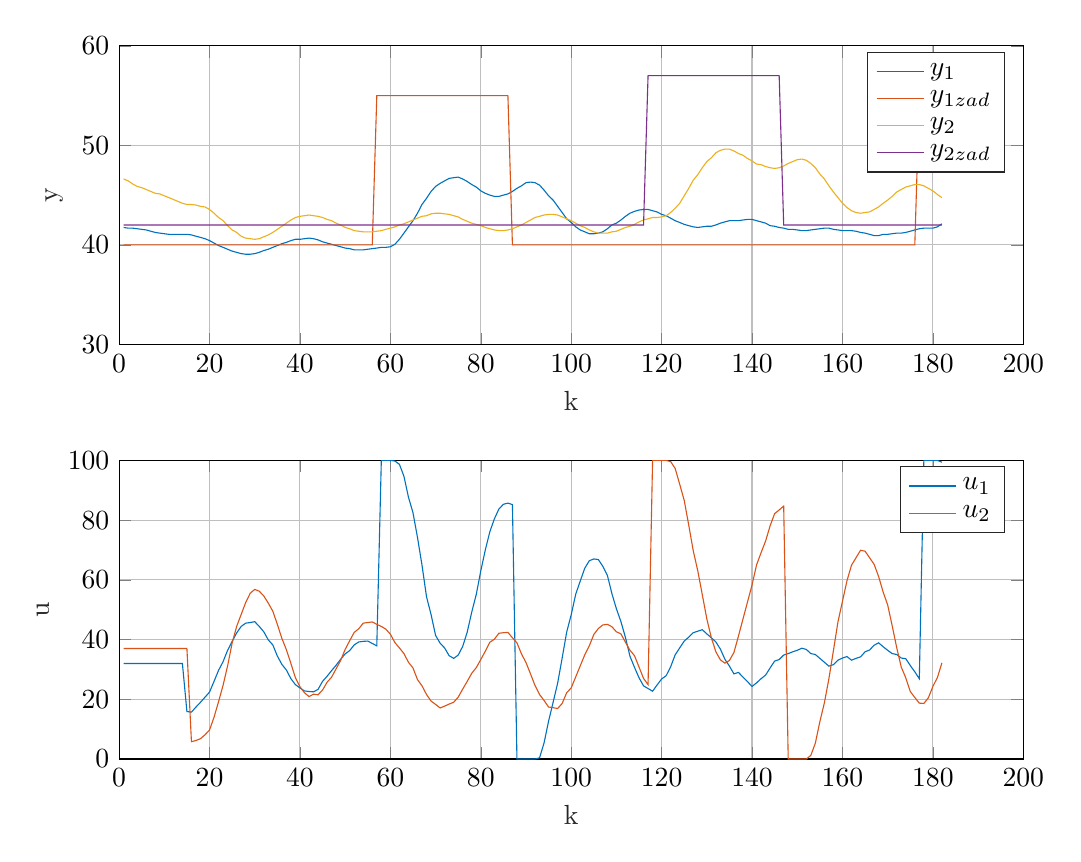
\begin{tikzpicture}

\begin{axis}[%
width=4.521in,
height=1.493in,
at={(0.758in,2.554in)},
scale only axis,
xmin=0,
xmax=200,
xlabel style={font=\color{white!15!black}},
xlabel={k},
ymin=30,
ymax=60,
ylabel style={font=\color{white!15!black}},
ylabel={y},
axis background/.style={fill=white},
xmajorgrids,
ymajorgrids,
legend style={legend cell align=left, align=left, draw=white!15!black}
]
\addplot [color=mycolor1]
  table[row sep=crcr]{%
1	41.75\\
2	41.68\\
3	41.68\\
4	41.62\\
5	41.56\\
6	41.5\\
7	41.37\\
8	41.25\\
9	41.18\\
10	41.12\\
11	41.06\\
12	41.06\\
13	41.06\\
14	41.06\\
15	41.06\\
16	41\\
17	40.87\\
18	40.75\\
19	40.62\\
20	40.43\\
21	40.18\\
22	39.93\\
23	39.75\\
24	39.56\\
25	39.37\\
26	39.25\\
27	39.12\\
28	39.06\\
29	39.06\\
30	39.12\\
31	39.25\\
32	39.43\\
33	39.56\\
34	39.75\\
35	39.93\\
36	40.12\\
37	40.25\\
38	40.43\\
39	40.56\\
40	40.56\\
41	40.62\\
42	40.68\\
43	40.62\\
44	40.5\\
45	40.31\\
46	40.18\\
47	40.06\\
48	39.93\\
49	39.81\\
50	39.68\\
51	39.62\\
52	39.5\\
53	39.5\\
54	39.5\\
55	39.56\\
56	39.62\\
57	39.68\\
58	39.75\\
59	39.75\\
60	39.81\\
61	40.06\\
62	40.56\\
63	41.18\\
64	41.81\\
65	42.43\\
66	43.18\\
67	44.06\\
68	44.68\\
69	45.37\\
70	45.87\\
71	46.18\\
72	46.43\\
73	46.68\\
74	46.75\\
75	46.81\\
76	46.62\\
77	46.37\\
78	46.06\\
79	45.81\\
80	45.43\\
81	45.18\\
82	45\\
83	44.87\\
84	44.87\\
85	45\\
86	45.12\\
87	45.37\\
88	45.68\\
89	45.93\\
90	46.25\\
91	46.31\\
92	46.25\\
93	46\\
94	45.5\\
95	44.93\\
96	44.5\\
97	43.87\\
98	43.25\\
99	42.62\\
100	42.25\\
101	41.81\\
102	41.5\\
103	41.31\\
104	41.12\\
105	41.12\\
106	41.18\\
107	41.31\\
108	41.62\\
109	42\\
110	42.18\\
111	42.5\\
112	42.87\\
113	43.18\\
114	43.37\\
115	43.5\\
116	43.56\\
117	43.56\\
118	43.43\\
119	43.31\\
120	43.06\\
121	42.93\\
122	42.68\\
123	42.43\\
124	42.25\\
125	42.06\\
126	41.93\\
127	41.81\\
128	41.75\\
129	41.81\\
130	41.87\\
131	41.87\\
132	42\\
133	42.18\\
134	42.31\\
135	42.43\\
136	42.43\\
137	42.43\\
138	42.5\\
139	42.56\\
140	42.56\\
141	42.43\\
142	42.31\\
143	42.18\\
144	41.93\\
145	41.87\\
146	41.75\\
147	41.68\\
148	41.56\\
149	41.56\\
150	41.5\\
151	41.43\\
152	41.43\\
153	41.5\\
154	41.56\\
155	41.62\\
156	41.68\\
157	41.68\\
158	41.56\\
159	41.5\\
160	41.43\\
161	41.43\\
162	41.43\\
163	41.37\\
164	41.25\\
165	41.18\\
166	41.06\\
167	40.93\\
168	40.93\\
169	41.06\\
170	41.06\\
171	41.12\\
172	41.18\\
173	41.18\\
174	41.25\\
175	41.37\\
176	41.5\\
177	41.62\\
178	41.68\\
179	41.68\\
180	41.68\\
181	41.81\\
182	42.12\\
};
\addlegendentry{$\text{y}_\text{1}$}

\addplot [color=mycolor2]
  table[row sep=crcr]{%
1	40\\
2	40\\
3	40\\
4	40\\
5	40\\
6	40\\
7	40\\
8	40\\
9	40\\
10	40\\
11	40\\
12	40\\
13	40\\
14	40\\
15	40\\
16	40\\
17	40\\
18	40\\
19	40\\
20	40\\
21	40\\
22	40\\
23	40\\
24	40\\
25	40\\
26	40\\
27	40\\
28	40\\
29	40\\
30	40\\
31	40\\
32	40\\
33	40\\
34	40\\
35	40\\
36	40\\
37	40\\
38	40\\
39	40\\
40	40\\
41	40\\
42	40\\
43	40\\
44	40\\
45	40\\
46	40\\
47	40\\
48	40\\
49	40\\
50	40\\
51	40\\
52	40\\
53	40\\
54	40\\
55	40\\
56	40\\
57	55\\
58	55\\
59	55\\
60	55\\
61	55\\
62	55\\
63	55\\
64	55\\
65	55\\
66	55\\
67	55\\
68	55\\
69	55\\
70	55\\
71	55\\
72	55\\
73	55\\
74	55\\
75	55\\
76	55\\
77	55\\
78	55\\
79	55\\
80	55\\
81	55\\
82	55\\
83	55\\
84	55\\
85	55\\
86	55\\
87	40\\
88	40\\
89	40\\
90	40\\
91	40\\
92	40\\
93	40\\
94	40\\
95	40\\
96	40\\
97	40\\
98	40\\
99	40\\
100	40\\
101	40\\
102	40\\
103	40\\
104	40\\
105	40\\
106	40\\
107	40\\
108	40\\
109	40\\
110	40\\
111	40\\
112	40\\
113	40\\
114	40\\
115	40\\
116	40\\
117	40\\
118	40\\
119	40\\
120	40\\
121	40\\
122	40\\
123	40\\
124	40\\
125	40\\
126	40\\
127	40\\
128	40\\
129	40\\
130	40\\
131	40\\
132	40\\
133	40\\
134	40\\
135	40\\
136	40\\
137	40\\
138	40\\
139	40\\
140	40\\
141	40\\
142	40\\
143	40\\
144	40\\
145	40\\
146	40\\
147	40\\
148	40\\
149	40\\
150	40\\
151	40\\
152	40\\
153	40\\
154	40\\
155	40\\
156	40\\
157	40\\
158	40\\
159	40\\
160	40\\
161	40\\
162	40\\
163	40\\
164	40\\
165	40\\
166	40\\
167	40\\
168	40\\
169	40\\
170	40\\
171	40\\
172	40\\
173	40\\
174	40\\
175	40\\
176	40\\
177	55\\
178	55\\
179	55\\
180	55\\
181	55\\
182	55\\
};
\addlegendentry{$\text{y}_{\text{1zad}}$}

\addplot [color=mycolor3]
  table[row sep=crcr]{%
1	46.62\\
2	46.43\\
3	46.12\\
4	45.87\\
5	45.75\\
6	45.56\\
7	45.37\\
8	45.18\\
9	45.12\\
10	44.93\\
11	44.75\\
12	44.56\\
13	44.37\\
14	44.18\\
15	44.06\\
16	44.06\\
17	44\\
18	43.87\\
19	43.81\\
20	43.56\\
21	43.18\\
22	42.75\\
23	42.43\\
24	41.93\\
25	41.5\\
26	41.25\\
27	40.87\\
28	40.68\\
29	40.62\\
30	40.56\\
31	40.62\\
32	40.81\\
33	41\\
34	41.25\\
35	41.56\\
36	41.87\\
37	42.18\\
38	42.5\\
39	42.75\\
40	42.87\\
41	42.93\\
42	43\\
43	42.93\\
44	42.87\\
45	42.75\\
46	42.56\\
47	42.43\\
48	42.18\\
49	42\\
50	41.75\\
51	41.62\\
52	41.43\\
53	41.37\\
54	41.31\\
55	41.31\\
56	41.31\\
57	41.37\\
58	41.43\\
59	41.56\\
60	41.68\\
61	41.81\\
62	42\\
63	42.12\\
64	42.31\\
65	42.5\\
66	42.68\\
67	42.87\\
68	42.93\\
69	43.12\\
70	43.18\\
71	43.18\\
72	43.12\\
73	43.06\\
74	42.93\\
75	42.81\\
76	42.56\\
77	42.37\\
78	42.18\\
79	42.06\\
80	41.93\\
81	41.75\\
82	41.62\\
83	41.5\\
84	41.43\\
85	41.43\\
86	41.5\\
87	41.62\\
88	41.81\\
89	42\\
90	42.25\\
91	42.5\\
92	42.75\\
93	42.87\\
94	43\\
95	43.06\\
96	43.06\\
97	43\\
98	42.81\\
99	42.62\\
100	42.43\\
101	42.18\\
102	41.93\\
103	41.75\\
104	41.5\\
105	41.31\\
106	41.18\\
107	41.18\\
108	41.18\\
109	41.31\\
110	41.37\\
111	41.56\\
112	41.75\\
113	41.87\\
114	42.06\\
115	42.31\\
116	42.5\\
117	42.62\\
118	42.75\\
119	42.75\\
120	42.81\\
121	42.93\\
122	43.25\\
123	43.68\\
124	44.18\\
125	44.93\\
126	45.68\\
127	46.5\\
128	47.06\\
129	47.75\\
130	48.37\\
131	48.75\\
132	49.25\\
133	49.5\\
134	49.62\\
135	49.62\\
136	49.43\\
137	49.18\\
138	49\\
139	48.68\\
140	48.43\\
141	48.12\\
142	48.06\\
143	47.87\\
144	47.75\\
145	47.68\\
146	47.75\\
147	47.93\\
148	48.18\\
149	48.37\\
150	48.56\\
151	48.62\\
152	48.5\\
153	48.18\\
154	47.75\\
155	47.12\\
156	46.62\\
157	45.93\\
158	45.31\\
159	44.75\\
160	44.18\\
161	43.75\\
162	43.43\\
163	43.25\\
164	43.18\\
165	43.25\\
166	43.31\\
167	43.56\\
168	43.81\\
169	44.18\\
170	44.5\\
171	44.87\\
172	45.31\\
173	45.56\\
174	45.81\\
175	45.93\\
176	46.06\\
177	46.06\\
178	45.93\\
179	45.68\\
180	45.43\\
181	45.06\\
182	44.75\\
};
\addlegendentry{$\text{y}_\text{2}$}

\addplot [color=mycolor4]
  table[row sep=crcr]{%
1	42\\
2	42\\
3	42\\
4	42\\
5	42\\
6	42\\
7	42\\
8	42\\
9	42\\
10	42\\
11	42\\
12	42\\
13	42\\
14	42\\
15	42\\
16	42\\
17	42\\
18	42\\
19	42\\
20	42\\
21	42\\
22	42\\
23	42\\
24	42\\
25	42\\
26	42\\
27	42\\
28	42\\
29	42\\
30	42\\
31	42\\
32	42\\
33	42\\
34	42\\
35	42\\
36	42\\
37	42\\
38	42\\
39	42\\
40	42\\
41	42\\
42	42\\
43	42\\
44	42\\
45	42\\
46	42\\
47	42\\
48	42\\
49	42\\
50	42\\
51	42\\
52	42\\
53	42\\
54	42\\
55	42\\
56	42\\
57	42\\
58	42\\
59	42\\
60	42\\
61	42\\
62	42\\
63	42\\
64	42\\
65	42\\
66	42\\
67	42\\
68	42\\
69	42\\
70	42\\
71	42\\
72	42\\
73	42\\
74	42\\
75	42\\
76	42\\
77	42\\
78	42\\
79	42\\
80	42\\
81	42\\
82	42\\
83	42\\
84	42\\
85	42\\
86	42\\
87	42\\
88	42\\
89	42\\
90	42\\
91	42\\
92	42\\
93	42\\
94	42\\
95	42\\
96	42\\
97	42\\
98	42\\
99	42\\
100	42\\
101	42\\
102	42\\
103	42\\
104	42\\
105	42\\
106	42\\
107	42\\
108	42\\
109	42\\
110	42\\
111	42\\
112	42\\
113	42\\
114	42\\
115	42\\
116	42\\
117	57\\
118	57\\
119	57\\
120	57\\
121	57\\
122	57\\
123	57\\
124	57\\
125	57\\
126	57\\
127	57\\
128	57\\
129	57\\
130	57\\
131	57\\
132	57\\
133	57\\
134	57\\
135	57\\
136	57\\
137	57\\
138	57\\
139	57\\
140	57\\
141	57\\
142	57\\
143	57\\
144	57\\
145	57\\
146	57\\
147	42\\
148	42\\
149	42\\
150	42\\
151	42\\
152	42\\
153	42\\
154	42\\
155	42\\
156	42\\
157	42\\
158	42\\
159	42\\
160	42\\
161	42\\
162	42\\
163	42\\
164	42\\
165	42\\
166	42\\
167	42\\
168	42\\
169	42\\
170	42\\
171	42\\
172	42\\
173	42\\
174	42\\
175	42\\
176	42\\
177	42\\
178	42\\
179	42\\
180	42\\
181	42\\
182	42\\
};
\addlegendentry{$\text{y}_{\text{2zad}}$}

\end{axis}

\begin{axis}[%
width=4.521in,
height=1.493in,
at={(0.758in,0.481in)},
scale only axis,
xmin=0,
xmax=200,
xlabel style={font=\color{white!15!black}},
xlabel={k},
ymin=0,
ymax=100,
ylabel style={font=\color{white!15!black}},
ylabel={u},
axis background/.style={fill=white},
xmajorgrids,
ymajorgrids,
legend style={legend cell align=left, align=left, draw=white!15!black}
]
\addplot [color=mycolor1]
  table[row sep=crcr]{%
1	32\\
2	32\\
3	32\\
4	32\\
5	32\\
6	32\\
7	32\\
8	32\\
9	32\\
10	32\\
11	32\\
12	32\\
13	32\\
14	32\\
15	15.9\\
16	15.7\\
17	17.4\\
18	19\\
19	20.7\\
20	22.4\\
21	26\\
22	29.7\\
23	32.6\\
24	36.4\\
25	39.4\\
26	42.2\\
27	44.4\\
28	45.5\\
29	45.7\\
30	46\\
31	44.4\\
32	42.6\\
33	39.9\\
34	38.2\\
35	34.5\\
36	31.7\\
37	29.8\\
38	26.9\\
39	24.9\\
40	23.8\\
41	22.8\\
42	22.6\\
43	22.5\\
44	23.3\\
45	26\\
46	27.7\\
47	29.6\\
48	31.4\\
49	33.4\\
50	35.2\\
51	36.3\\
52	38.2\\
53	39.2\\
54	39.4\\
55	39.5\\
56	38.7\\
57	37.9\\
58	100\\
59	100\\
60	100\\
61	99.8\\
62	98.7\\
63	94.7\\
64	87.7\\
65	82.5\\
66	74.2\\
67	64.9\\
68	54.3\\
69	48.4\\
70	41.4\\
71	38.8\\
72	37.2\\
73	34.6\\
74	33.7\\
75	34.8\\
76	37.7\\
77	42.5\\
78	49.2\\
79	55.1\\
80	63\\
81	70\\
82	76.1\\
83	80.4\\
84	83.7\\
85	85.3\\
86	85.7\\
87	85.2\\
88	0\\
89	0\\
90	0\\
91	0\\
92	0\\
93	0.4\\
94	5.4\\
95	12.7\\
96	19\\
97	25.4\\
98	33.8\\
99	42.5\\
100	48.3\\
101	55.2\\
102	59.6\\
103	63.9\\
104	66.4\\
105	67\\
106	66.8\\
107	64.5\\
108	61.5\\
109	55.4\\
110	50.3\\
111	46\\
112	40.7\\
113	34.4\\
114	30.7\\
115	27.2\\
116	24.5\\
117	23.6\\
118	22.7\\
119	24.8\\
120	26.8\\
121	27.9\\
122	30.9\\
123	34.9\\
124	37.2\\
125	39.5\\
126	40.8\\
127	42.3\\
128	42.8\\
129	43.3\\
130	41.9\\
131	40.6\\
132	39.2\\
133	36.8\\
134	33.4\\
135	31.1\\
136	28.5\\
137	29\\
138	27.4\\
139	25.9\\
140	24.3\\
141	25.5\\
142	26.9\\
143	28.1\\
144	30.5\\
145	32.8\\
146	33.3\\
147	34.8\\
148	35.3\\
149	35.9\\
150	36.4\\
151	37.1\\
152	36.7\\
153	35.3\\
154	35\\
155	33.7\\
156	32.4\\
157	31.1\\
158	31.6\\
159	33.1\\
160	33.8\\
161	34.3\\
162	33.1\\
163	33.7\\
164	34.2\\
165	35.9\\
166	36.5\\
167	38.1\\
168	38.9\\
169	37.6\\
170	36.4\\
171	35.3\\
172	35\\
173	33.8\\
174	33.6\\
175	31.3\\
176	29.2\\
177	26.9\\
178	100\\
179	100\\
180	100\\
181	100\\
182	99.4\\
};
\addlegendentry{$\text{u}_\text{1}$}

\addplot [color=mycolor2]
  table[row sep=crcr]{%
1	37\\
2	37\\
3	37\\
4	37\\
5	37\\
6	37\\
7	37\\
8	37\\
9	37\\
10	37\\
11	37\\
12	37\\
13	37\\
14	37\\
15	37\\
16	5.8\\
17	6.2\\
18	6.8\\
19	8.1\\
20	9.7\\
21	14\\
22	19.2\\
23	24.7\\
24	31.2\\
25	38.8\\
26	44.4\\
27	48.4\\
28	52.4\\
29	55.5\\
30	56.8\\
31	56.2\\
32	54.6\\
33	52.2\\
34	49.5\\
35	45.1\\
36	40.4\\
37	36.6\\
38	32\\
39	27.2\\
40	24.2\\
41	22.2\\
42	20.9\\
43	21.7\\
44	21.5\\
45	23.1\\
46	25.7\\
47	27.4\\
48	30.2\\
49	33\\
50	36.7\\
51	39.6\\
52	42.4\\
53	43.6\\
54	45.5\\
55	45.7\\
56	45.9\\
57	45.1\\
58	44.4\\
59	43.5\\
60	41.8\\
61	39\\
62	37.2\\
63	35.3\\
64	32.4\\
65	30.5\\
66	26.6\\
67	24.5\\
68	21.6\\
69	19.4\\
70	18.3\\
71	17.1\\
72	17.7\\
73	18.4\\
74	19\\
75	20.7\\
76	23.4\\
77	26\\
78	28.7\\
79	30.6\\
80	33.3\\
81	36.1\\
82	39.1\\
83	40.1\\
84	42.1\\
85	42.3\\
86	42.4\\
87	40.6\\
88	38.9\\
89	35.2\\
90	32.3\\
91	28.5\\
92	24.6\\
93	21.6\\
94	19.6\\
95	17.4\\
96	17.2\\
97	16.9\\
98	18.6\\
99	22.2\\
100	23.8\\
101	27.5\\
102	31.2\\
103	34.9\\
104	37.9\\
105	41.7\\
106	43.7\\
107	44.9\\
108	45.1\\
109	44.3\\
110	42.6\\
111	41.9\\
112	39.1\\
113	36.4\\
114	34.6\\
115	30.8\\
116	27\\
117	24.9\\
118	100\\
119	100\\
120	100\\
121	100\\
122	99.6\\
123	97.3\\
124	92\\
125	86.6\\
126	78.3\\
127	69.7\\
128	63\\
129	55\\
130	46.9\\
131	40.6\\
132	35.9\\
133	33.2\\
134	32.1\\
135	33\\
136	35.7\\
137	41.2\\
138	46.9\\
139	52.6\\
140	58.3\\
141	65\\
142	69.1\\
143	73\\
144	78.1\\
145	82.2\\
146	83.4\\
147	84.7\\
148	0\\
149	0\\
150	0\\
151	0\\
152	0\\
153	1.2\\
154	5.3\\
155	12.5\\
156	18.8\\
157	26.9\\
158	36.3\\
159	45.9\\
160	52.8\\
161	59.7\\
162	64.9\\
163	67.4\\
164	69.9\\
165	69.6\\
166	67.4\\
167	65.2\\
168	61.1\\
169	55.9\\
170	51.6\\
171	44.6\\
172	37.3\\
173	30.8\\
174	27.2\\
175	22.6\\
176	20.6\\
177	18.7\\
178	18.6\\
179	20.5\\
180	24.3\\
181	27.3\\
182	32.2\\
};
\addlegendentry{$\text{u}_{\text{2}}$}

\end{axis}
\end{tikzpicture}%
    \caption{Eksperyment z regulatorem P}
    \label{lab:zad3:figure:regulatorP}
 \end{figure}
 \fi

 $$Kr = \num{30.0} \indent Ti = \num{25.0} \indent Td = \num{0.001}$$

\ifdefined\CompileFigures
\begin{figure}[H] 
    \centering
    % This file was created by matlab2tikz.
%
\definecolor{mycolor1}{rgb}{0.00000,0.44700,0.74100}%
\definecolor{mycolor2}{rgb}{0.85000,0.32500,0.09800}%
\definecolor{mycolor3}{rgb}{0.92900,0.69400,0.12500}%
\definecolor{mycolor4}{rgb}{0.49400,0.18400,0.55600}%
%
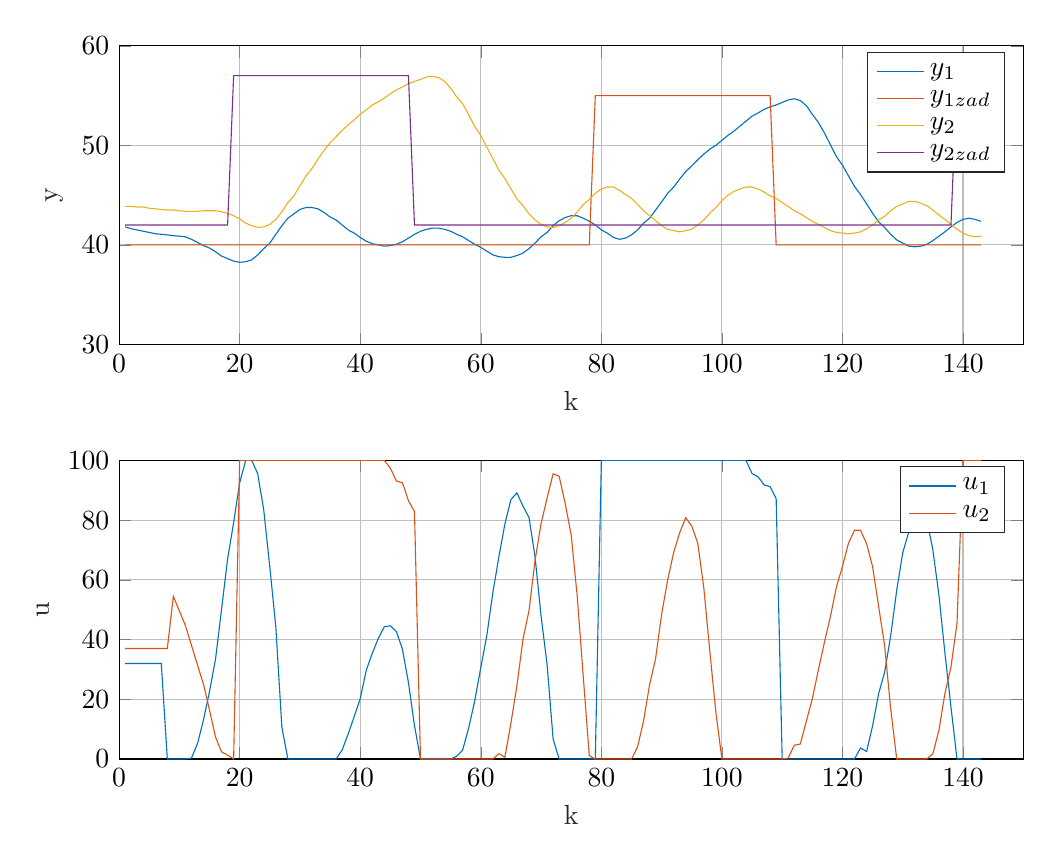
\begin{tikzpicture}

\begin{axis}[%
width=4.521in,
height=1.493in,
at={(0.758in,2.554in)},
scale only axis,
xmin=0,
xmax=150,
xlabel style={font=\color{white!15!black}},
xlabel={k},
ymin=30,
ymax=60,
ylabel style={font=\color{white!15!black}},
ylabel={y},
axis background/.style={fill=white},
xmajorgrids,
ymajorgrids,
legend style={legend cell align=left, align=left, draw=white!15!black}
]
\addplot [color=mycolor1]
  table[row sep=crcr]{%
1	41.81\\
2	41.62\\
3	41.5\\
4	41.37\\
5	41.25\\
6	41.12\\
7	41.06\\
8	41\\
9	40.93\\
10	40.87\\
11	40.81\\
12	40.56\\
13	40.25\\
14	39.93\\
15	39.68\\
16	39.31\\
17	38.87\\
18	38.62\\
19	38.37\\
20	38.25\\
21	38.31\\
22	38.5\\
23	39\\
24	39.62\\
25	40.18\\
26	41.06\\
27	41.93\\
28	42.68\\
29	43.12\\
30	43.56\\
31	43.75\\
32	43.75\\
33	43.62\\
34	43.25\\
35	42.81\\
36	42.5\\
37	42\\
38	41.5\\
39	41.18\\
40	40.75\\
41	40.37\\
42	40.12\\
43	40\\
44	39.87\\
45	39.93\\
46	40.06\\
47	40.31\\
48	40.68\\
49	41.06\\
50	41.37\\
51	41.56\\
52	41.68\\
53	41.68\\
54	41.56\\
55	41.37\\
56	41.06\\
57	40.81\\
58	40.43\\
59	40.06\\
60	39.75\\
61	39.37\\
62	39\\
63	38.81\\
64	38.75\\
65	38.75\\
66	38.93\\
67	39.18\\
68	39.62\\
69	40.18\\
70	40.81\\
71	41.25\\
72	41.93\\
73	42.43\\
74	42.75\\
75	42.93\\
76	42.93\\
77	42.68\\
78	42.37\\
79	42\\
80	41.5\\
81	41.18\\
82	40.75\\
83	40.56\\
84	40.68\\
85	41\\
86	41.5\\
87	42.18\\
88	42.68\\
89	43.5\\
90	44.31\\
91	45.18\\
92	45.81\\
93	46.62\\
94	47.37\\
95	47.93\\
96	48.56\\
97	49.12\\
98	49.62\\
99	50\\
100	50.5\\
101	51\\
102	51.43\\
103	51.93\\
104	52.43\\
105	52.93\\
106	53.25\\
107	53.62\\
108	53.87\\
109	54.06\\
110	54.31\\
111	54.56\\
112	54.68\\
113	54.5\\
114	54\\
115	53.12\\
116	52.31\\
117	51.25\\
118	50.06\\
119	48.87\\
120	48\\
121	46.93\\
122	45.87\\
123	45.06\\
124	44.12\\
125	43.18\\
126	42.31\\
127	41.75\\
128	41.06\\
129	40.5\\
130	40.18\\
131	39.87\\
132	39.81\\
133	39.87\\
134	40.06\\
135	40.43\\
136	40.87\\
137	41.31\\
138	41.81\\
139	42.25\\
140	42.56\\
141	42.68\\
142	42.56\\
143	42.37\\
};
\addlegendentry{$\text{y}_\text{1}$}

\addplot [color=mycolor2]
  table[row sep=crcr]{%
1	40\\
2	40\\
3	40\\
4	40\\
5	40\\
6	40\\
7	40\\
8	40\\
9	40\\
10	40\\
11	40\\
12	40\\
13	40\\
14	40\\
15	40\\
16	40\\
17	40\\
18	40\\
19	40\\
20	40\\
21	40\\
22	40\\
23	40\\
24	40\\
25	40\\
26	40\\
27	40\\
28	40\\
29	40\\
30	40\\
31	40\\
32	40\\
33	40\\
34	40\\
35	40\\
36	40\\
37	40\\
38	40\\
39	40\\
40	40\\
41	40\\
42	40\\
43	40\\
44	40\\
45	40\\
46	40\\
47	40\\
48	40\\
49	40\\
50	40\\
51	40\\
52	40\\
53	40\\
54	40\\
55	40\\
56	40\\
57	40\\
58	40\\
59	40\\
60	40\\
61	40\\
62	40\\
63	40\\
64	40\\
65	40\\
66	40\\
67	40\\
68	40\\
69	40\\
70	40\\
71	40\\
72	40\\
73	40\\
74	40\\
75	40\\
76	40\\
77	40\\
78	40\\
79	55\\
80	55\\
81	55\\
82	55\\
83	55\\
84	55\\
85	55\\
86	55\\
87	55\\
88	55\\
89	55\\
90	55\\
91	55\\
92	55\\
93	55\\
94	55\\
95	55\\
96	55\\
97	55\\
98	55\\
99	55\\
100	55\\
101	55\\
102	55\\
103	55\\
104	55\\
105	55\\
106	55\\
107	55\\
108	55\\
109	40\\
110	40\\
111	40\\
112	40\\
113	40\\
114	40\\
115	40\\
116	40\\
117	40\\
118	40\\
119	40\\
120	40\\
121	40\\
122	40\\
123	40\\
124	40\\
125	40\\
126	40\\
127	40\\
128	40\\
129	40\\
130	40\\
131	40\\
132	40\\
133	40\\
134	40\\
135	40\\
136	40\\
137	40\\
138	40\\
139	40\\
140	40\\
141	40\\
142	40\\
143	40\\
};
\addlegendentry{$\text{y}_{\text{1zad}}$}

\addplot [color=mycolor3]
  table[row sep=crcr]{%
1	43.87\\
2	43.87\\
3	43.81\\
4	43.81\\
5	43.68\\
6	43.62\\
7	43.56\\
8	43.5\\
9	43.5\\
10	43.43\\
11	43.37\\
12	43.37\\
13	43.37\\
14	43.43\\
15	43.43\\
16	43.43\\
17	43.31\\
18	43.18\\
19	42.93\\
20	42.62\\
21	42.18\\
22	41.93\\
23	41.75\\
24	41.81\\
25	42.06\\
26	42.56\\
27	43.31\\
28	44.25\\
29	44.93\\
30	45.93\\
31	46.93\\
32	47.68\\
33	48.62\\
34	49.5\\
35	50.25\\
36	50.87\\
37	51.5\\
38	52.06\\
39	52.56\\
40	53.12\\
41	53.56\\
42	54.06\\
43	54.37\\
44	54.75\\
45	55.18\\
46	55.56\\
47	55.87\\
48	56.18\\
49	56.43\\
50	56.62\\
51	56.87\\
52	56.93\\
53	56.81\\
54	56.43\\
55	55.75\\
56	54.87\\
57	54.18\\
58	53.06\\
59	51.87\\
60	51\\
61	49.81\\
62	48.68\\
63	47.5\\
64	46.68\\
65	45.62\\
66	44.62\\
67	43.93\\
68	43.12\\
69	42.5\\
70	42.06\\
71	41.81\\
72	41.75\\
73	41.93\\
74	42.25\\
75	42.68\\
76	43.31\\
77	44.06\\
78	44.56\\
79	45.18\\
80	45.62\\
81	45.81\\
82	45.81\\
83	45.5\\
84	45.06\\
85	44.68\\
86	44.06\\
87	43.43\\
88	42.93\\
89	42.43\\
90	41.93\\
91	41.56\\
92	41.43\\
93	41.31\\
94	41.43\\
95	41.56\\
96	42\\
97	42.5\\
98	43.18\\
99	43.75\\
100	44.43\\
101	45\\
102	45.37\\
103	45.62\\
104	45.81\\
105	45.81\\
106	45.62\\
107	45.31\\
108	44.93\\
109	44.68\\
110	44.25\\
111	43.87\\
112	43.43\\
113	43.12\\
114	42.75\\
115	42.37\\
116	42.06\\
117	41.75\\
118	41.43\\
119	41.25\\
120	41.18\\
121	41.12\\
122	41.18\\
123	41.31\\
124	41.62\\
125	42\\
126	42.5\\
127	42.87\\
128	43.43\\
129	43.87\\
130	44.12\\
131	44.37\\
132	44.37\\
133	44.18\\
134	43.93\\
135	43.5\\
136	43\\
137	42.56\\
138	42.06\\
139	41.56\\
140	41.18\\
141	40.93\\
142	40.81\\
143	40.87\\
};
\addlegendentry{$\text{y}_\text{2}$}

\addplot [color=mycolor4]
  table[row sep=crcr]{%
1	42\\
2	42\\
3	42\\
4	42\\
5	42\\
6	42\\
7	42\\
8	42\\
9	42\\
10	42\\
11	42\\
12	42\\
13	42\\
14	42\\
15	42\\
16	42\\
17	42\\
18	42\\
19	57\\
20	57\\
21	57\\
22	57\\
23	57\\
24	57\\
25	57\\
26	57\\
27	57\\
28	57\\
29	57\\
30	57\\
31	57\\
32	57\\
33	57\\
34	57\\
35	57\\
36	57\\
37	57\\
38	57\\
39	57\\
40	57\\
41	57\\
42	57\\
43	57\\
44	57\\
45	57\\
46	57\\
47	57\\
48	57\\
49	42\\
50	42\\
51	42\\
52	42\\
53	42\\
54	42\\
55	42\\
56	42\\
57	42\\
58	42\\
59	42\\
60	42\\
61	42\\
62	42\\
63	42\\
64	42\\
65	42\\
66	42\\
67	42\\
68	42\\
69	42\\
70	42\\
71	42\\
72	42\\
73	42\\
74	42\\
75	42\\
76	42\\
77	42\\
78	42\\
79	42\\
80	42\\
81	42\\
82	42\\
83	42\\
84	42\\
85	42\\
86	42\\
87	42\\
88	42\\
89	42\\
90	42\\
91	42\\
92	42\\
93	42\\
94	42\\
95	42\\
96	42\\
97	42\\
98	42\\
99	42\\
100	42\\
101	42\\
102	42\\
103	42\\
104	42\\
105	42\\
106	42\\
107	42\\
108	42\\
109	42\\
110	42\\
111	42\\
112	42\\
113	42\\
114	42\\
115	42\\
116	42\\
117	42\\
118	42\\
119	42\\
120	42\\
121	42\\
122	42\\
123	42\\
124	42\\
125	42\\
126	42\\
127	42\\
128	42\\
129	42\\
130	42\\
131	42\\
132	42\\
133	42\\
134	42\\
135	42\\
136	42\\
137	42\\
138	42\\
139	57\\
140	57\\
141	57\\
142	57\\
143	57\\
};
\addlegendentry{$\text{y}_{\text{2zad}}$}

\end{axis}

\begin{axis}[%
width=4.521in,
height=1.493in,
at={(0.758in,0.481in)},
scale only axis,
xmin=0,
xmax=150,
xlabel style={font=\color{white!15!black}},
xlabel={k},
ymin=0,
ymax=100,
ylabel style={font=\color{white!15!black}},
ylabel={u},
axis background/.style={fill=white},
xmajorgrids,
ymajorgrids,
legend style={legend cell align=left, align=left, draw=white!15!black}
]
\addplot [color=mycolor1]
  table[row sep=crcr]{%
1	32\\
2	32\\
3	32\\
4	32\\
5	32\\
6	32\\
7	32\\
8	0\\
9	0\\
10	0\\
11	0\\
12	0.3\\
13	5.1\\
14	13.1\\
15	22.6\\
16	33.5\\
17	50.2\\
18	67\\
19	79.2\\
20	92.5\\
21	100\\
22	100\\
23	95.5\\
24	83.3\\
25	64.3\\
26	44.2\\
27	10.7\\
28	0\\
29	0\\
30	0\\
31	0\\
32	0\\
33	0\\
34	0\\
35	0\\
36	0\\
37	3\\
38	8.4\\
39	14.2\\
40	20.2\\
41	29.7\\
42	35.4\\
43	40.4\\
44	44.3\\
45	44.6\\
46	42.7\\
47	36.8\\
48	25.6\\
49	11.2\\
50	0\\
51	0\\
52	0\\
53	0\\
54	0\\
55	0\\
56	0.9\\
57	3\\
58	10.5\\
59	19.5\\
60	30.6\\
61	41.3\\
62	55.7\\
63	67.7\\
64	78.7\\
65	86.9\\
66	89.1\\
67	84.7\\
68	80.9\\
69	67.7\\
70	47.9\\
71	31.6\\
72	6.7\\
73	0\\
74	0\\
75	0\\
76	0\\
77	0\\
78	0\\
79	0\\
80	100\\
81	100\\
82	100\\
83	100\\
84	100\\
85	100\\
86	100\\
87	100\\
88	100\\
89	100\\
90	100\\
91	100\\
92	100\\
93	100\\
94	100\\
95	100\\
96	100\\
97	100\\
98	100\\
99	100\\
100	100\\
101	100\\
102	100\\
103	100\\
104	100\\
105	95.6\\
106	94.5\\
107	91.8\\
108	91.2\\
109	87.2\\
110	0\\
111	0\\
112	0\\
113	0\\
114	0\\
115	0\\
116	0\\
117	0\\
118	0\\
119	0\\
120	0\\
121	0\\
122	0\\
123	3.7\\
124	2.5\\
125	11.1\\
126	21.9\\
127	29.1\\
128	41.3\\
129	56.5\\
130	69.1\\
131	76\\
132	82.1\\
133	83\\
134	80.1\\
135	70\\
136	54.9\\
137	35.4\\
138	17.4\\
139	0\\
140	0\\
141	0\\
142	0\\
143	0\\
};
\addlegendentry{$\text{u}_\text{1}$}

\addplot [color=mycolor2]
  table[row sep=crcr]{%
1	37\\
2	37\\
3	37\\
4	37\\
5	37\\
6	37\\
7	37\\
8	37\\
9	54.5\\
10	49.6\\
11	44.7\\
12	38.1\\
13	31.5\\
14	25\\
15	16.4\\
16	7.3\\
17	2.4\\
18	1.3\\
19	0\\
20	100\\
21	100\\
22	100\\
23	100\\
24	100\\
25	100\\
26	100\\
27	100\\
28	100\\
29	100\\
30	100\\
31	100\\
32	100\\
33	100\\
34	100\\
35	100\\
36	100\\
37	100\\
38	100\\
39	100\\
40	100\\
41	100\\
42	100\\
43	100\\
44	100\\
45	97.4\\
46	93.1\\
47	92.5\\
48	86.5\\
49	82.9\\
50	0\\
51	0\\
52	0\\
53	0\\
54	0\\
55	0\\
56	0\\
57	0\\
58	0\\
59	0\\
60	0\\
61	0\\
62	0\\
63	1.8\\
64	0.6\\
65	12\\
66	24.6\\
67	40.1\\
68	49.7\\
69	66.5\\
70	78.8\\
71	87.4\\
72	95.5\\
73	94.7\\
74	85.6\\
75	75\\
76	54.5\\
77	27.6\\
78	1.1\\
79	0\\
80	0\\
81	0\\
82	0\\
83	0\\
84	0\\
85	0\\
86	4\\
87	12.7\\
88	24.8\\
89	33.6\\
90	48.5\\
91	59.9\\
92	69.2\\
93	75.8\\
94	80.8\\
95	78\\
96	72.3\\
97	57.3\\
98	36\\
99	15.6\\
100	0\\
101	0\\
102	0\\
103	0\\
104	0\\
105	0\\
106	0\\
107	0\\
108	0\\
109	0\\
110	0\\
111	0.3\\
112	4.6\\
113	5\\
114	12.6\\
115	20.2\\
116	29.8\\
117	39\\
118	47.7\\
119	57.6\\
120	64.5\\
121	72.3\\
122	76.6\\
123	76.6\\
124	72.1\\
125	64.4\\
126	51.1\\
127	37.9\\
128	16.8\\
129	0\\
130	0\\
131	0\\
132	0\\
133	0\\
134	0\\
135	1.8\\
136	9.6\\
137	22\\
138	30.8\\
139	45.5\\
140	100\\
141	100\\
142	100\\
143	100\\
};
\addlegendentry{$\text{u}_{\text{2}}$}

\end{axis}
\end{tikzpicture}%
    \caption{Eksperyment z regulatorem PI}
    \label{lab:zad3:figure:regulatorPI}
 \end{figure}
 \fi

 $$Kr = \num{30.0} \indent Ti = \num{25.0} \indent Td = \num{1}$$

\ifdefined\CompileFigures
\begin{figure}[H] 
    \centering
    % This file was created by matlab2tikz.
%
\definecolor{mycolor1}{rgb}{0.00000,0.44700,0.74100}%
\definecolor{mycolor2}{rgb}{0.85000,0.32500,0.09800}%
\definecolor{mycolor3}{rgb}{0.92900,0.69400,0.12500}%
\definecolor{mycolor4}{rgb}{0.49400,0.18400,0.55600}%
%
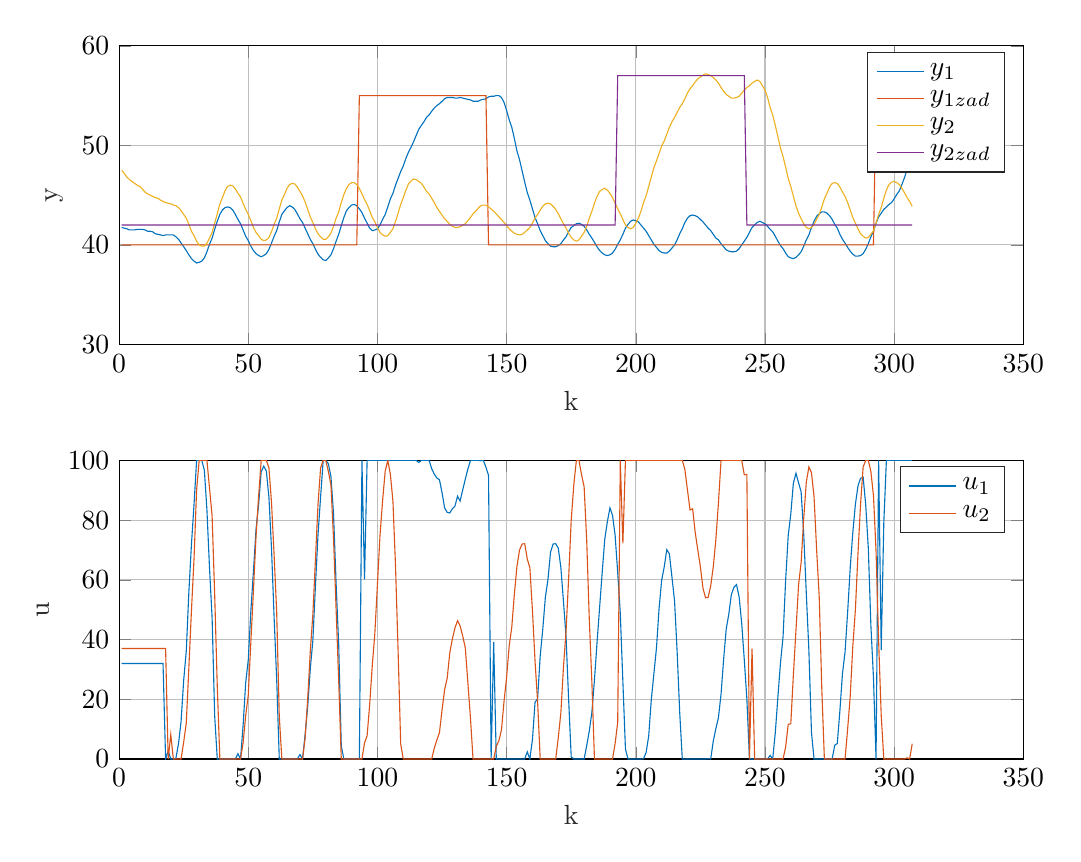
\begin{tikzpicture}

\begin{axis}[%
width=4.521in,
height=1.493in,
at={(0.758in,2.554in)},
scale only axis,
xmin=0,
xmax=350,
xlabel style={font=\color{white!15!black}},
xlabel={k},
ymin=30,
ymax=60,
ylabel style={font=\color{white!15!black}},
ylabel={y},
axis background/.style={fill=white},
xmajorgrids,
ymajorgrids,
legend style={legend cell align=left, align=left, draw=white!15!black}
]
\addplot [color=mycolor1]
  table[row sep=crcr]{%
1	41.75\\
2	41.68\\
3	41.62\\
4	41.5\\
5	41.5\\
6	41.5\\
7	41.56\\
8	41.56\\
9	41.56\\
10	41.5\\
11	41.37\\
12	41.37\\
13	41.31\\
14	41.12\\
15	41.06\\
16	41\\
17	40.93\\
18	41\\
19	41\\
20	41\\
21	41\\
22	40.81\\
23	40.56\\
24	40.18\\
25	39.81\\
26	39.43\\
27	39\\
28	38.62\\
29	38.37\\
30	38.18\\
31	38.25\\
32	38.37\\
33	38.68\\
34	39.31\\
35	40.06\\
36	40.68\\
37	41.56\\
38	42.37\\
39	43.06\\
40	43.5\\
41	43.75\\
42	43.81\\
43	43.75\\
44	43.5\\
45	43.06\\
46	42.56\\
47	42.12\\
48	41.5\\
49	40.87\\
50	40.43\\
51	39.87\\
52	39.43\\
53	39.12\\
54	38.93\\
55	38.81\\
56	38.93\\
57	39.12\\
58	39.56\\
59	40.18\\
60	40.87\\
61	41.43\\
62	42.31\\
63	43.06\\
64	43.43\\
65	43.75\\
66	43.93\\
67	43.81\\
68	43.56\\
69	43.12\\
70	42.62\\
71	42.25\\
72	41.68\\
73	41.12\\
74	40.56\\
75	40.12\\
76	39.56\\
77	39.06\\
78	38.75\\
79	38.5\\
80	38.43\\
81	38.68\\
82	39\\
83	39.62\\
84	40.37\\
85	41.06\\
86	41.93\\
87	42.75\\
88	43.43\\
89	43.75\\
90	44\\
91	44.06\\
92	43.93\\
93	43.62\\
94	43.25\\
95	42.68\\
96	42.18\\
97	41.68\\
98	41.43\\
99	41.5\\
100	41.62\\
101	42\\
102	42.56\\
103	43.06\\
104	43.81\\
105	44.62\\
106	45.18\\
107	46\\
108	46.68\\
109	47.37\\
110	47.93\\
111	48.68\\
112	49.31\\
113	49.81\\
114	50.37\\
115	51\\
116	51.62\\
117	52\\
118	52.37\\
119	52.81\\
120	53.06\\
121	53.43\\
122	53.75\\
123	54\\
124	54.18\\
125	54.43\\
126	54.68\\
127	54.81\\
128	54.81\\
129	54.81\\
130	54.75\\
131	54.75\\
132	54.81\\
133	54.75\\
134	54.68\\
135	54.62\\
136	54.56\\
137	54.43\\
138	54.43\\
139	54.43\\
140	54.56\\
141	54.62\\
142	54.68\\
143	54.87\\
144	54.93\\
145	54.93\\
146	55\\
147	55\\
148	54.81\\
149	54.31\\
150	53.5\\
151	52.56\\
152	51.81\\
153	50.68\\
154	49.43\\
155	48.56\\
156	47.43\\
157	46.31\\
158	45.25\\
159	44.5\\
160	43.62\\
161	42.75\\
162	42.12\\
163	41.43\\
164	40.93\\
165	40.43\\
166	40.12\\
167	39.87\\
168	39.81\\
169	39.81\\
170	39.93\\
171	40.12\\
172	40.5\\
173	40.81\\
174	41.31\\
175	41.75\\
176	41.93\\
177	42.12\\
178	42.18\\
179	42.06\\
180	41.87\\
181	41.5\\
182	41.06\\
183	40.68\\
184	40.25\\
185	39.81\\
186	39.43\\
187	39.18\\
188	39\\
189	38.93\\
190	39\\
191	39.18\\
192	39.56\\
193	40.06\\
194	40.5\\
195	41.06\\
196	41.68\\
197	42.06\\
198	42.37\\
199	42.5\\
200	42.43\\
201	42.31\\
202	42\\
203	41.68\\
204	41.37\\
205	40.93\\
206	40.5\\
207	40.06\\
208	39.75\\
209	39.43\\
210	39.25\\
211	39.18\\
212	39.18\\
213	39.37\\
214	39.68\\
215	40\\
216	40.5\\
217	41.12\\
218	41.62\\
219	42.25\\
220	42.68\\
221	42.93\\
222	43\\
223	42.93\\
224	42.81\\
225	42.56\\
226	42.31\\
227	42\\
228	41.68\\
229	41.43\\
230	41.06\\
231	40.68\\
232	40.5\\
233	40.12\\
234	39.81\\
235	39.5\\
236	39.37\\
237	39.31\\
238	39.31\\
239	39.37\\
240	39.62\\
241	40\\
242	40.37\\
243	40.75\\
244	41.25\\
245	41.75\\
246	42\\
247	42.25\\
248	42.37\\
249	42.25\\
250	42.12\\
251	41.87\\
252	41.56\\
253	41.31\\
254	40.87\\
255	40.37\\
256	39.93\\
257	39.62\\
258	39.18\\
259	38.81\\
260	38.68\\
261	38.62\\
262	38.75\\
263	39\\
264	39.31\\
265	39.87\\
266	40.5\\
267	41\\
268	41.75\\
269	42.37\\
270	42.87\\
271	43.12\\
272	43.31\\
273	43.31\\
274	43.18\\
275	42.93\\
276	42.56\\
277	42.06\\
278	41.68\\
279	41.06\\
280	40.56\\
281	40.18\\
282	39.75\\
283	39.37\\
284	39.06\\
285	38.87\\
286	38.87\\
287	38.93\\
288	39.12\\
289	39.56\\
290	40.12\\
291	40.81\\
292	41.37\\
293	42.18\\
294	42.81\\
295	43.18\\
296	43.56\\
297	43.81\\
298	44.06\\
299	44.25\\
300	44.62\\
301	45.06\\
302	45.43\\
303	46.06\\
304	46.75\\
305	47.56\\
306	48.12\\
307	48.87\\
};
\addlegendentry{$\text{y}_\text{1}$}

\addplot [color=mycolor2]
  table[row sep=crcr]{%
1	40\\
2	40\\
3	40\\
4	40\\
5	40\\
6	40\\
7	40\\
8	40\\
9	40\\
10	40\\
11	40\\
12	40\\
13	40\\
14	40\\
15	40\\
16	40\\
17	40\\
18	40\\
19	40\\
20	40\\
21	40\\
22	40\\
23	40\\
24	40\\
25	40\\
26	40\\
27	40\\
28	40\\
29	40\\
30	40\\
31	40\\
32	40\\
33	40\\
34	40\\
35	40\\
36	40\\
37	40\\
38	40\\
39	40\\
40	40\\
41	40\\
42	40\\
43	40\\
44	40\\
45	40\\
46	40\\
47	40\\
48	40\\
49	40\\
50	40\\
51	40\\
52	40\\
53	40\\
54	40\\
55	40\\
56	40\\
57	40\\
58	40\\
59	40\\
60	40\\
61	40\\
62	40\\
63	40\\
64	40\\
65	40\\
66	40\\
67	40\\
68	40\\
69	40\\
70	40\\
71	40\\
72	40\\
73	40\\
74	40\\
75	40\\
76	40\\
77	40\\
78	40\\
79	40\\
80	40\\
81	40\\
82	40\\
83	40\\
84	40\\
85	40\\
86	40\\
87	40\\
88	40\\
89	40\\
90	40\\
91	40\\
92	40\\
93	55\\
94	55\\
95	55\\
96	55\\
97	55\\
98	55\\
99	55\\
100	55\\
101	55\\
102	55\\
103	55\\
104	55\\
105	55\\
106	55\\
107	55\\
108	55\\
109	55\\
110	55\\
111	55\\
112	55\\
113	55\\
114	55\\
115	55\\
116	55\\
117	55\\
118	55\\
119	55\\
120	55\\
121	55\\
122	55\\
123	55\\
124	55\\
125	55\\
126	55\\
127	55\\
128	55\\
129	55\\
130	55\\
131	55\\
132	55\\
133	55\\
134	55\\
135	55\\
136	55\\
137	55\\
138	55\\
139	55\\
140	55\\
141	55\\
142	55\\
143	40\\
144	40\\
145	40\\
146	40\\
147	40\\
148	40\\
149	40\\
150	40\\
151	40\\
152	40\\
153	40\\
154	40\\
155	40\\
156	40\\
157	40\\
158	40\\
159	40\\
160	40\\
161	40\\
162	40\\
163	40\\
164	40\\
165	40\\
166	40\\
167	40\\
168	40\\
169	40\\
170	40\\
171	40\\
172	40\\
173	40\\
174	40\\
175	40\\
176	40\\
177	40\\
178	40\\
179	40\\
180	40\\
181	40\\
182	40\\
183	40\\
184	40\\
185	40\\
186	40\\
187	40\\
188	40\\
189	40\\
190	40\\
191	40\\
192	40\\
193	40\\
194	40\\
195	40\\
196	40\\
197	40\\
198	40\\
199	40\\
200	40\\
201	40\\
202	40\\
203	40\\
204	40\\
205	40\\
206	40\\
207	40\\
208	40\\
209	40\\
210	40\\
211	40\\
212	40\\
213	40\\
214	40\\
215	40\\
216	40\\
217	40\\
218	40\\
219	40\\
220	40\\
221	40\\
222	40\\
223	40\\
224	40\\
225	40\\
226	40\\
227	40\\
228	40\\
229	40\\
230	40\\
231	40\\
232	40\\
233	40\\
234	40\\
235	40\\
236	40\\
237	40\\
238	40\\
239	40\\
240	40\\
241	40\\
242	40\\
243	40\\
244	40\\
245	40\\
246	40\\
247	40\\
248	40\\
249	40\\
250	40\\
251	40\\
252	40\\
253	40\\
254	40\\
255	40\\
256	40\\
257	40\\
258	40\\
259	40\\
260	40\\
261	40\\
262	40\\
263	40\\
264	40\\
265	40\\
266	40\\
267	40\\
268	40\\
269	40\\
270	40\\
271	40\\
272	40\\
273	40\\
274	40\\
275	40\\
276	40\\
277	40\\
278	40\\
279	40\\
280	40\\
281	40\\
282	40\\
283	40\\
284	40\\
285	40\\
286	40\\
287	40\\
288	40\\
289	40\\
290	40\\
291	40\\
292	40\\
293	55\\
294	55\\
295	55\\
296	55\\
297	55\\
298	55\\
299	55\\
300	55\\
301	55\\
302	55\\
303	55\\
304	55\\
305	55\\
306	55\\
307	55\\
};
\addlegendentry{$\text{y}_{\text{1zad}}$}

\addplot [color=mycolor3]
  table[row sep=crcr]{%
1	47.5\\
2	47.18\\
3	46.81\\
4	46.56\\
5	46.37\\
6	46.18\\
7	46\\
8	45.87\\
9	45.62\\
10	45.31\\
11	45.12\\
12	45\\
13	44.87\\
14	44.75\\
15	44.68\\
16	44.5\\
17	44.37\\
18	44.25\\
19	44.18\\
20	44.12\\
21	44\\
22	43.93\\
23	43.75\\
24	43.43\\
25	43.06\\
26	42.68\\
27	42.06\\
28	41.37\\
29	40.93\\
30	40.37\\
31	40\\
32	39.87\\
33	39.87\\
34	40.18\\
35	40.68\\
36	41.25\\
37	42.18\\
38	43.12\\
39	44.12\\
40	44.75\\
41	45.43\\
42	45.87\\
43	46\\
44	45.93\\
45	45.62\\
46	45.18\\
47	44.81\\
48	44.18\\
49	43.56\\
50	43.06\\
51	42.43\\
52	41.75\\
53	41.25\\
54	40.93\\
55	40.56\\
56	40.43\\
57	40.5\\
58	40.75\\
59	41.31\\
60	42.06\\
61	42.68\\
62	43.62\\
63	44.5\\
64	45.06\\
65	45.68\\
66	46.06\\
67	46.18\\
68	46.12\\
69	45.81\\
70	45.37\\
71	44.93\\
72	44.31\\
73	43.56\\
74	42.81\\
75	42.25\\
76	41.62\\
77	41.12\\
78	40.81\\
79	40.56\\
80	40.56\\
81	40.81\\
82	41.18\\
83	41.87\\
84	42.68\\
85	43.31\\
86	44.25\\
87	45.06\\
88	45.68\\
89	46.06\\
90	46.25\\
91	46.25\\
92	46.06\\
93	45.68\\
94	45.12\\
95	44.56\\
96	44.06\\
97	43.43\\
98	42.75\\
99	42.31\\
100	41.75\\
101	41.25\\
102	41\\
103	40.87\\
104	40.93\\
105	41.25\\
106	41.62\\
107	42.37\\
108	43.18\\
109	44.06\\
110	44.75\\
111	45.5\\
112	46.12\\
113	46.43\\
114	46.62\\
115	46.56\\
116	46.37\\
117	46.18\\
118	45.81\\
119	45.37\\
120	45.12\\
121	44.68\\
122	44.25\\
123	43.75\\
124	43.37\\
125	43\\
126	42.62\\
127	42.37\\
128	42.06\\
129	41.87\\
130	41.75\\
131	41.75\\
132	41.81\\
133	42\\
134	42.12\\
135	42.43\\
136	42.75\\
137	43.12\\
138	43.37\\
139	43.68\\
140	43.93\\
141	44\\
142	44\\
143	43.81\\
144	43.62\\
145	43.37\\
146	43.12\\
147	42.81\\
148	42.56\\
149	42.25\\
150	41.93\\
151	41.62\\
152	41.37\\
153	41.18\\
154	41.06\\
155	41\\
156	41.06\\
157	41.25\\
158	41.5\\
159	41.75\\
160	42.18\\
161	42.68\\
162	43.06\\
163	43.5\\
164	43.87\\
165	44.12\\
166	44.18\\
167	44.12\\
168	43.87\\
169	43.56\\
170	43.12\\
171	42.62\\
172	42.12\\
173	41.68\\
174	41.18\\
175	40.75\\
176	40.5\\
177	40.37\\
178	40.5\\
179	40.87\\
180	41.25\\
181	41.87\\
182	42.68\\
183	43.37\\
184	44.18\\
185	44.87\\
186	45.37\\
187	45.56\\
188	45.68\\
189	45.5\\
190	45.18\\
191	44.75\\
192	44.18\\
193	43.62\\
194	43.12\\
195	42.56\\
196	42\\
197	41.75\\
198	41.62\\
199	41.75\\
200	42.18\\
201	42.68\\
202	43.37\\
203	44.25\\
204	44.93\\
205	45.87\\
206	46.81\\
207	47.75\\
208	48.43\\
209	49.18\\
210	49.93\\
211	50.43\\
212	51.12\\
213	51.81\\
214	52.37\\
215	52.81\\
216	53.31\\
217	53.81\\
218	54.18\\
219	54.68\\
220	55.25\\
221	55.68\\
222	56\\
223	56.37\\
224	56.68\\
225	56.87\\
226	57.06\\
227	57.18\\
228	57.12\\
229	57\\
230	56.81\\
231	56.56\\
232	56.25\\
233	55.81\\
234	55.43\\
235	55.12\\
236	54.93\\
237	54.75\\
238	54.75\\
239	54.81\\
240	54.93\\
241	55.25\\
242	55.56\\
243	55.81\\
244	56\\
245	56.25\\
246	56.43\\
247	56.56\\
248	56.43\\
249	56\\
250	55.56\\
251	54.81\\
252	53.81\\
253	53.06\\
254	52\\
255	50.87\\
256	49.75\\
257	48.87\\
258	47.81\\
259	46.68\\
260	45.87\\
261	44.87\\
262	43.93\\
263	43.18\\
264	42.62\\
265	42.12\\
266	41.75\\
267	41.62\\
268	41.75\\
269	42.06\\
270	42.56\\
271	43.06\\
272	43.81\\
273	44.62\\
274	45.18\\
275	45.81\\
276	46.18\\
277	46.25\\
278	46.18\\
279	45.81\\
280	45.31\\
281	44.87\\
282	44.25\\
283	43.5\\
284	42.75\\
285	42.18\\
286	41.62\\
287	41.12\\
288	40.87\\
289	40.68\\
290	40.75\\
291	41.06\\
292	41.43\\
293	42.18\\
294	43.06\\
295	43.75\\
296	44.68\\
297	45.5\\
298	46.06\\
299	46.31\\
300	46.37\\
301	46.25\\
302	46.06\\
303	45.68\\
304	45.25\\
305	44.75\\
306	44.37\\
307	43.87\\
};
\addlegendentry{$\text{y}_\text{2}$}

\addplot [color=mycolor4]
  table[row sep=crcr]{%
1	42\\
2	42\\
3	42\\
4	42\\
5	42\\
6	42\\
7	42\\
8	42\\
9	42\\
10	42\\
11	42\\
12	42\\
13	42\\
14	42\\
15	42\\
16	42\\
17	42\\
18	42\\
19	42\\
20	42\\
21	42\\
22	42\\
23	42\\
24	42\\
25	42\\
26	42\\
27	42\\
28	42\\
29	42\\
30	42\\
31	42\\
32	42\\
33	42\\
34	42\\
35	42\\
36	42\\
37	42\\
38	42\\
39	42\\
40	42\\
41	42\\
42	42\\
43	42\\
44	42\\
45	42\\
46	42\\
47	42\\
48	42\\
49	42\\
50	42\\
51	42\\
52	42\\
53	42\\
54	42\\
55	42\\
56	42\\
57	42\\
58	42\\
59	42\\
60	42\\
61	42\\
62	42\\
63	42\\
64	42\\
65	42\\
66	42\\
67	42\\
68	42\\
69	42\\
70	42\\
71	42\\
72	42\\
73	42\\
74	42\\
75	42\\
76	42\\
77	42\\
78	42\\
79	42\\
80	42\\
81	42\\
82	42\\
83	42\\
84	42\\
85	42\\
86	42\\
87	42\\
88	42\\
89	42\\
90	42\\
91	42\\
92	42\\
93	42\\
94	42\\
95	42\\
96	42\\
97	42\\
98	42\\
99	42\\
100	42\\
101	42\\
102	42\\
103	42\\
104	42\\
105	42\\
106	42\\
107	42\\
108	42\\
109	42\\
110	42\\
111	42\\
112	42\\
113	42\\
114	42\\
115	42\\
116	42\\
117	42\\
118	42\\
119	42\\
120	42\\
121	42\\
122	42\\
123	42\\
124	42\\
125	42\\
126	42\\
127	42\\
128	42\\
129	42\\
130	42\\
131	42\\
132	42\\
133	42\\
134	42\\
135	42\\
136	42\\
137	42\\
138	42\\
139	42\\
140	42\\
141	42\\
142	42\\
143	42\\
144	42\\
145	42\\
146	42\\
147	42\\
148	42\\
149	42\\
150	42\\
151	42\\
152	42\\
153	42\\
154	42\\
155	42\\
156	42\\
157	42\\
158	42\\
159	42\\
160	42\\
161	42\\
162	42\\
163	42\\
164	42\\
165	42\\
166	42\\
167	42\\
168	42\\
169	42\\
170	42\\
171	42\\
172	42\\
173	42\\
174	42\\
175	42\\
176	42\\
177	42\\
178	42\\
179	42\\
180	42\\
181	42\\
182	42\\
183	42\\
184	42\\
185	42\\
186	42\\
187	42\\
188	42\\
189	42\\
190	42\\
191	42\\
192	42\\
193	57\\
194	57\\
195	57\\
196	57\\
197	57\\
198	57\\
199	57\\
200	57\\
201	57\\
202	57\\
203	57\\
204	57\\
205	57\\
206	57\\
207	57\\
208	57\\
209	57\\
210	57\\
211	57\\
212	57\\
213	57\\
214	57\\
215	57\\
216	57\\
217	57\\
218	57\\
219	57\\
220	57\\
221	57\\
222	57\\
223	57\\
224	57\\
225	57\\
226	57\\
227	57\\
228	57\\
229	57\\
230	57\\
231	57\\
232	57\\
233	57\\
234	57\\
235	57\\
236	57\\
237	57\\
238	57\\
239	57\\
240	57\\
241	57\\
242	57\\
243	42\\
244	42\\
245	42\\
246	42\\
247	42\\
248	42\\
249	42\\
250	42\\
251	42\\
252	42\\
253	42\\
254	42\\
255	42\\
256	42\\
257	42\\
258	42\\
259	42\\
260	42\\
261	42\\
262	42\\
263	42\\
264	42\\
265	42\\
266	42\\
267	42\\
268	42\\
269	42\\
270	42\\
271	42\\
272	42\\
273	42\\
274	42\\
275	42\\
276	42\\
277	42\\
278	42\\
279	42\\
280	42\\
281	42\\
282	42\\
283	42\\
284	42\\
285	42\\
286	42\\
287	42\\
288	42\\
289	42\\
290	42\\
291	42\\
292	42\\
293	42\\
294	42\\
295	42\\
296	42\\
297	42\\
298	42\\
299	42\\
300	42\\
301	42\\
302	42\\
303	42\\
304	42\\
305	42\\
306	42\\
307	42\\
};
\addlegendentry{$\text{y}_{\text{2zad}}$}

\end{axis}

\begin{axis}[%
width=4.521in,
height=1.493in,
at={(0.758in,0.481in)},
scale only axis,
xmin=0,
xmax=350,
xlabel style={font=\color{white!15!black}},
xlabel={k},
ymin=0,
ymax=100,
ylabel style={font=\color{white!15!black}},
ylabel={u},
axis background/.style={fill=white},
xmajorgrids,
ymajorgrids,
legend style={legend cell align=left, align=left, draw=white!15!black}
]
\addplot [color=mycolor1]
  table[row sep=crcr]{%
1	32\\
2	32\\
3	32\\
4	32\\
5	32\\
6	32\\
7	32\\
8	32\\
9	32\\
10	32\\
11	32\\
12	32\\
13	32\\
14	32\\
15	32\\
16	32\\
17	32\\
18	0\\
19	2.7\\
20	0\\
21	0\\
22	0.3\\
23	5.2\\
24	12.7\\
25	26.4\\
26	36.1\\
27	55.9\\
28	71.8\\
29	85.2\\
30	100\\
31	100\\
32	100\\
33	96.7\\
34	83.3\\
35	63.9\\
36	47.3\\
37	14.4\\
38	0\\
39	0\\
40	0\\
41	0\\
42	0\\
43	0\\
44	0\\
45	0\\
46	1.8\\
47	0\\
48	11.2\\
49	25.6\\
50	33.2\\
51	49.6\\
52	62.9\\
53	76.9\\
54	85.2\\
55	96.2\\
56	98.1\\
57	96.4\\
58	87.6\\
59	70.3\\
60	47.5\\
61	26.6\\
62	0\\
63	0\\
64	0\\
65	0\\
66	0\\
67	0\\
68	0\\
69	0\\
70	1.5\\
71	0\\
72	8.1\\
73	17.5\\
74	30.1\\
75	39.7\\
76	58\\
77	75.2\\
78	87.8\\
79	100\\
80	100\\
81	98.9\\
82	94.6\\
83	82.1\\
84	58.7\\
85	38.3\\
86	4.4\\
87	0\\
88	0\\
89	0\\
90	0\\
91	0\\
92	0\\
93	0\\
94	100\\
95	60.2\\
96	100\\
97	100\\
98	100\\
99	100\\
100	100\\
101	100\\
102	100\\
103	100\\
104	100\\
105	100\\
106	100\\
107	100\\
108	100\\
109	100\\
110	100\\
111	100\\
112	100\\
113	100\\
114	100\\
115	100\\
116	99.3\\
117	100\\
118	100\\
119	100\\
120	100\\
121	97.2\\
122	95.4\\
123	94.1\\
124	93.5\\
125	89.2\\
126	84.1\\
127	82.6\\
128	82.4\\
129	83.8\\
130	84.7\\
131	88\\
132	86.4\\
133	90.1\\
134	93.7\\
135	97.1\\
136	100\\
137	100\\
138	100\\
139	100\\
140	99.9\\
141	100\\
142	97.7\\
143	95\\
144	0\\
145	39.1\\
146	0\\
147	0\\
148	0\\
149	0\\
150	0\\
151	0\\
152	0\\
153	0\\
154	0\\
155	0\\
156	0\\
157	0\\
158	2.4\\
159	0\\
160	6.6\\
161	19\\
162	20.2\\
163	34.5\\
164	43.5\\
165	54.2\\
166	60.1\\
167	69.3\\
168	72\\
169	72.1\\
170	70.6\\
171	64.1\\
172	52.8\\
173	41\\
174	20.1\\
175	0.7\\
176	0\\
177	0\\
178	0\\
179	0\\
180	0\\
181	4.5\\
182	9.4\\
183	15.6\\
184	26.5\\
185	39\\
186	50.8\\
187	62.5\\
188	73.7\\
189	79.5\\
190	84.1\\
191	81.6\\
192	74.9\\
193	62.4\\
194	48.8\\
195	25.9\\
196	3.3\\
197	0\\
198	0\\
199	0\\
200	0\\
201	0\\
202	0\\
203	0.1\\
204	2.2\\
205	7.7\\
206	19.8\\
207	28.5\\
208	37.1\\
209	50.2\\
210	59.8\\
211	64.3\\
212	70.1\\
213	68.7\\
214	60.9\\
215	53\\
216	36\\
217	15.6\\
218	0\\
219	0\\
220	0\\
221	0\\
222	0\\
223	0\\
224	0\\
225	0\\
226	0\\
227	0\\
228	0.1\\
229	0\\
230	6\\
231	10.2\\
232	13.9\\
233	21.7\\
234	33.4\\
235	43.5\\
236	48.5\\
237	55.1\\
238	57.5\\
239	58.4\\
240	54.3\\
241	45.4\\
242	33.2\\
243	20.1\\
244	0\\
245	0\\
246	0\\
247	0\\
248	0\\
249	0\\
250	0\\
251	0\\
252	1.2\\
253	0\\
254	8.8\\
255	20.7\\
256	32.1\\
257	40.9\\
258	59.8\\
259	74.8\\
260	82.1\\
261	92.4\\
262	95.7\\
263	92.5\\
264	89.5\\
265	75.4\\
266	55.5\\
267	36.4\\
268	8.9\\
269	0\\
270	0\\
271	0\\
272	0\\
273	0\\
274	0\\
275	0\\
276	0\\
277	4.6\\
278	5.2\\
279	16.1\\
280	28.6\\
281	35.8\\
282	49.1\\
283	64\\
284	75.8\\
285	85.3\\
286	91.4\\
287	94\\
288	94.4\\
289	85.1\\
290	70.7\\
291	44.8\\
292	27.2\\
293	0\\
294	100\\
295	36.5\\
296	79.1\\
297	100\\
298	100\\
299	100\\
300	100\\
301	100\\
302	100\\
303	100\\
304	100\\
305	100\\
306	100\\
307	100\\
};
\addlegendentry{$\text{u}_\text{1}$}

\addplot [color=mycolor2]
  table[row sep=crcr]{%
1	37\\
2	37\\
3	37\\
4	37\\
5	37\\
6	37\\
7	37\\
8	37\\
9	37\\
10	37\\
11	37\\
12	37\\
13	37\\
14	37\\
15	37\\
16	37\\
17	37\\
18	37\\
19	0\\
20	8.2\\
21	0\\
22	0\\
23	0\\
24	0\\
25	5.7\\
26	12\\
27	30.5\\
28	49.6\\
29	67\\
30	90.1\\
31	100\\
32	100\\
33	100\\
34	100\\
35	90.7\\
36	81.4\\
37	55\\
38	24.4\\
39	0\\
40	0\\
41	0\\
42	0\\
43	0\\
44	0\\
45	0\\
46	0\\
47	0\\
48	5.4\\
49	14.5\\
50	21.4\\
51	39.2\\
52	56.5\\
53	74.5\\
54	88\\
55	100\\
56	100\\
57	100\\
58	97.5\\
59	85.8\\
60	68.3\\
61	49.2\\
62	14.3\\
63	0\\
64	0\\
65	0\\
66	0\\
67	0\\
68	0\\
69	0\\
70	0\\
71	0\\
72	6.9\\
73	20.1\\
74	36\\
75	48.4\\
76	66.8\\
77	85.4\\
78	97.5\\
79	100\\
80	100\\
81	96.3\\
82	91.8\\
83	73.9\\
84	50.1\\
85	26.2\\
86	0\\
87	0\\
88	0\\
89	0\\
90	0\\
91	0\\
92	0\\
93	0\\
94	0\\
95	5.4\\
96	7.8\\
97	18.3\\
98	31.3\\
99	42.1\\
100	58.6\\
101	75\\
102	86.6\\
103	96.4\\
104	100\\
105	95.4\\
106	86.3\\
107	64.5\\
108	36\\
109	5\\
110	0\\
111	0\\
112	0\\
113	0\\
114	0\\
115	0\\
116	0\\
117	0\\
118	0\\
119	0\\
120	0\\
121	0\\
122	3.6\\
123	6.4\\
124	8.8\\
125	16.4\\
126	23.2\\
127	27.1\\
128	35.5\\
129	40.2\\
130	43.9\\
131	46.3\\
132	44.6\\
133	41.2\\
134	37.3\\
135	25.6\\
136	13.8\\
137	0\\
138	0\\
139	0\\
140	0\\
141	0\\
142	0\\
143	0\\
144	0\\
145	0\\
146	4.2\\
147	6.1\\
148	9.7\\
149	19.3\\
150	27.4\\
151	37.9\\
152	44.2\\
153	55.2\\
154	64.5\\
155	70\\
156	72\\
157	72.1\\
158	67\\
159	64\\
160	49.7\\
161	32.8\\
162	19.1\\
163	0\\
164	0\\
165	0\\
166	0\\
167	0\\
168	0\\
169	0\\
170	7.2\\
171	15.5\\
172	30.7\\
173	42.8\\
174	60.4\\
175	79.9\\
176	91.8\\
177	100\\
178	100\\
179	95.2\\
180	91.2\\
181	73.3\\
182	46.8\\
183	25.8\\
184	0\\
185	0\\
186	0\\
187	0\\
188	0\\
189	0\\
190	0\\
191	0\\
192	5.2\\
193	12.3\\
194	100\\
195	72.2\\
196	100\\
197	100\\
198	100\\
199	100\\
200	100\\
201	100\\
202	100\\
203	100\\
204	100\\
205	100\\
206	100\\
207	100\\
208	100\\
209	100\\
210	100\\
211	100\\
212	100\\
213	100\\
214	100\\
215	100\\
216	100\\
217	100\\
218	100\\
219	97\\
220	90.1\\
221	83.4\\
222	83.8\\
223	75.9\\
224	70\\
225	64.4\\
226	57.2\\
227	54\\
228	54.1\\
229	58\\
230	64.4\\
231	73.6\\
232	85.9\\
233	100\\
234	100\\
235	100\\
236	100\\
237	100\\
238	100\\
239	100\\
240	100\\
241	100\\
242	95.2\\
243	95.3\\
244	0\\
245	37\\
246	0\\
247	0\\
248	0\\
249	0\\
250	0\\
251	0\\
252	0\\
253	0\\
254	0\\
255	0\\
256	0\\
257	0\\
258	4\\
259	11.6\\
260	11.8\\
261	28.2\\
262	43.1\\
263	58.2\\
264	65.8\\
265	80.5\\
266	92.7\\
267	97.8\\
268	95.9\\
269	87.9\\
270	70.1\\
271	54.3\\
272	23.5\\
273	0\\
274	0\\
275	0\\
276	0\\
277	0\\
278	0\\
279	0\\
280	0\\
281	0\\
282	10\\
283	21\\
284	37.7\\
285	49.9\\
286	68.7\\
287	85.2\\
288	97.8\\
289	100\\
290	100\\
291	96.3\\
292	88.2\\
293	69.6\\
294	39.5\\
295	14.6\\
296	0\\
297	0\\
298	0\\
299	0\\
300	0\\
301	0\\
302	0\\
303	0\\
304	0\\
305	0.4\\
306	0\\
307	5.1\\
};
\addlegendentry{$\text{u}_{\text{2}}$}

\end{axis}
\end{tikzpicture}%
    \caption{Eksperyment z regulatorem PID}
    \label{lab:zad3:figure:regulatorPID}
 \end{figure}
 \fi

\newpage
